
\documentclass[10pt,a4paper]{article}
% \documentclass[12pt]{iopart} 
% \usepackage{iopams,setstack} 

\usepackage{graphicx}
\usepackage{algorithm, algorithmicx, algpseudocode} 
\usepackage{color} 
%This is to decrease the space in subfigure command
\usepackage[tight,scriptsize]{subfigure}
\makeatletter
\renewcommand{\subfigtopskip}{1\p@}
\renewcommand{\subfigcapskip}{0\p@}
\renewcommand{\subfigcaptopadj}{1\p@}
\renewcommand{\subfigbottomskip}{1\p@}
\renewcommand{\subfiglabelskip}{0.05em plus 0.02em minus 0.01em}
\makeatother
\renewcommand{\subcapsize}{\small}

% maths
\usepackage{amssymb,amsfonts,amsmath}
% notes
\newcommand{\parham}[1]{\textsf{\emph{\textbf{\textcolor{blue}{#1}}}}} 
\newcommand{\mike}[1]{\textsf{\emph{\textbf{\textcolor{red}{#1}}}}} 
\newcommand{\dean}[1]{\textsf{\emph{\textbf{\textcolor{green}{#1}}}}}
\newcommand{\ken}[1]{\textsf{\emph{\textbf{\textcolor{magenta}{#1}}}}}

\begin{document}

\title{State and Parameter Estimation for Spatio-Temporal Neural Fields}

\author{Dean R. Freestone$^{1,5}$, Parham Aram$^2$, Michael Dewar$^3$, Kenneth Scerri$^4$, \\David B. Grayden$^{1,5}$, and Visakan Kadirkamanathan$^2$}

% \address{$^1$ Department of Electrical and Electronic Engineering, University of Melbourne, Melbourne, VIC 3010 Australia} \address{$^2$ Department of Automatic Control and Systems Engineering, University of Sheffield, Mappin Street, Sheffield, S1 3JD, UK} \address{$^3$ Department of Applied Physics and Applied Mathematics, Columbia University, NY, USA} \address{$^4$ Department of Systems and Control Engineering, University of Malta, Msida, MSD 1333, Malta} \address{$^5$ The Bionic Ear Institute, East Melbourne, VIC 3002Australia} \ead{dfreestone@bionicear.org} 

\maketitle

\begin{abstract}
	This paper presents a framework for creating patient-specific neural field models from electrophysiological data. The Wilson and Cowen or Amari style neural field equations are used to form a parametric model, where the parameters are estimated from data. To illustrate the estimation framework, data is generated using the neural field equations incorporating modelled sensors, so a comparison can be made between estimated and true parameters. To facilitate state and parameter estimation, we introduce a method to reduce the continuum neural field model, using a basis function decomposition, to form a finite-dimensional state-space model. Spatial frequency analysis methods are introduced for model selection by systematically specifying the basis function configuration required to capture the dominant characteristics of the neural field. The estimation procedure consists of a two-stage iterative algorithm incorporating the unscented Rauch Tung Striebel Smoother for state estimation and a least squares algorithm for parameter estimation. The results show that it is possible to reconstruct the neural field and estimate intracortical connectivity and synaptic dynamics with the proposed framework. The results also illustrate the loss of high spatial frequency information as the cost incurred by the model reduction procedure. This framework provides a link between patient-specific neurophysiological data and theoretical neural fields models. This link may lead to greater understanding of cortical dynamics at the meso/macroscopic scale where diseases such as epilepsy are manifested.   
\end{abstract}

\section{Introduction} 

Generating physiologically plausible neural field models are of great importance for studying brain dynamics at the meso/macroscopic scale. While our understanding of the function of neurons is well developed, the overall behaviour of the brain's meso and macro-scale dynamics remains largely theoretical. Understanding the brain at this level is extremely important since it is at this scale that pathologies such as epilepsy, Parkinson's disease and schizophrenia are manifested. 

Mathematical neural field models provide insights into the underlying physics and dynamics of electroencephalography (EEG) and magnetoencephalography (MEG) (see \cite{Deco2008,David2003} for recent reviews). These models have demonstrated possible mechanisms for the genesis of neural rhythms (such as the alpha and gamma rhythms) \cite{Liley1999,RENNIE2000}, epileptic seizure generation \cite{DaSilva2003,Suffczynski2004,Wendling2005} and insights into other pathologies \cite{Moran2008,Schiff2009} that would be difficult to gain from experimental data alone. 

Unfortunately, the use of these models in the clinic has been limited, since they are constructed for ``general'' brain dynamics whereas pathologies almost always have unique underlying patient-specific causes. Patient-specific data from EEG is readily available in the clinical setting, suggesting an opportunity to make the patient-specific link to models of cortical dynamics. Furthermore, recent technological advances have driven an increased level of sophistication in recording techniques, with dramatic increases in spatial and temporal sampling~\cite{Brinkmann2009}. However, the meso/macroscopic neural dynamic state is not directly observable in EEG data, making predictions of the underlying physiology inherently difficult.

For models to be clinically viable, they must be patient-specific. A possible approach to achieve this would be to fit a general continuum neural field model, like the Wilson and Cohen (WC)~\cite{Wilson1973} or Amari~\cite{Amari1977} models or a neural mass model like the Jansen and Ritt model~\cite{Jansen1995}, to patient-specific EEG data. Fitting the neural models to individuals is a highly non-trivial task and, until very recently, has not been reported in the literature. 

An estimation framework for neural field models known as dynamical causal modelling (DCM) \cite{David2003,David2006} has recently been proposed for studying evoked potential dynamics. Via a Bayesian inference scheme, DCM estimates the long range (cortico-cortical) connectivity structure between the specific isolated brain regions that best explains a given data set using the Jansen and Ritt equations. Another recent publication describing a parameter estimation method with a neural field model used an unscented Kalman filter with the WC neural field equations~\cite{schiff2008kalman}. This work takes a system theoretic approach to the neural estimation problem, successfully demonstrating that it is possible to perform state estimation of modified WC equations. This marks the first step in what has the potential to revolutionise the treatment of many neurological diseases where therapeutic electrical stimulation is viable.

%Currently available epileptic seizure control devices (i.e., the vagal nerve stimulator) are implemented in an ``open loop". That is, the therapeutic electrical stimulation waveforms are adjusted for each patient by trial and error, disregarding the patient's neuro-dynamics and information about their particular pathologies. Given access to an accurate model, the application of optimal control theory in these circumstances would allow for robust therapeutic stimulations.

We present an extension to the work of Schiff and Sauer~\cite{schiff2008kalman} by establishing a framework for estimating the state of the WC equations for larger scale (more space) systems via a systematic model reduction procedure. In addition, a method is presented for estimating the connectivity structure and the synaptic time constant. Until now, estimation of local intracortical connectivity structure has not been reported (to the best of the authors' knowledge). Our work builds on recent work which shows that it is possible to estimate local coupling of spatiotemporal systems using techniques from control systems theory and machine learning~\cite{Dewar2009}. The key development here was to represent the spatiotemporal system as a standard state-space model, with the number of states independent of the number of observation locations (recording electrodes in this case). In addition, the appropriate model selection tools have been developed~\cite{Scerri2009} allowing for the application of the technique to neural fields. 

Modelling the neural dynamics within this framework has a distinct advantage over the more standard multivariate auto-regressive (AR) models: the number of parameters to define the spatial connectivity is considerably smaller than the number of AR coefficients typically required to achieve the required model complexity. 

In this paper, we demonstrate for the first time how intracortical connectivity can be inferred from data, based on a variant of the WC neural field model~\cite{Wilson1973}. This work provides a fundamental link between the theoretical advances in neural field modelling and patient-specific data.

The paper proceeds by first deriving the continuum neural field equations in Section~\ref{NeuralModelSection}. Then a finite dimensional neural field model is derived. The model is reduced by approximating the neural field using a set of continuous basis functions, weighted by a finite dimensional state vector. Section~\ref{SpectralAnalysisSection} establishes conditions using spatial frequency analysis for both sensor and basis function spacing and width, such that the dominant dynamics of the neural field can be represented by the reduced model. The state and parameter estimation procedure is described in Section~\ref{StateAndParameterEstimationSection}. The results for the spatial frequency analysis and parameter estimation are then presented in Section~\ref{ResultsSection}. The implications and limitations of this framework are discussed in Section~\ref{DiscussionSection} along with planned future developments.

\section{Neural Field Model}\label{NeuralModelSection} 

Neural field models relate mean firing rates of pre-synaptic neural populations to mean post-synaptic membrane potentials. They are popular as they are parsimonious yet have a strong link with the underlying physiology. Each neural population represents a functional cortical processing unit, such as a column. The columnar organisation of the cortex is continuous, where pyramidal cells are members of many columns. In general, cortical structure can be modelled in a physiologically plausible manner as being locally homogeneous (in short range intracortical connectivity) and heterogeneous (in long range cortico-cortical and corticothalamic connectivity)~\cite{Jirsa2009,Qubbaj2007}. In certain regions of the cortex, each column is thought to be connected locally via symmetric short range local excitation with surround inhibition \cite{Braitenberg1998}. For example, this structural organisation is most studied in the visual system, where the surrounding inhibition effectively tunes a cortical column to a particular receptive visual field~\cite{Sullivan2006}. Neural field models are descriptive of a range of neurodynamics of the cortex such as evoked potentials, visual hallucinations and epileptic behaviour~\cite{David2003,Bressloff2001,Breakspear2006}. Field models are also capable of generating complex spatial patterns of activity such as Turing patterns, spirals and travelling oscillations~\cite{Amari1977,Coombes2005,Coombes2007}.

\subsection{Derivation of the Integro-Difference Equation Representation}
The model relates the average number of action potentials $g(\mathbf{r},t)$ arriving at position $\mathbf{r}$ to the local post-synaptic membrane voltage $v(\mathbf{r},t)$. The post-synaptic potentials generated at a neuronal population at location $\mathbf{r}$ by action potentials arriving from all other connected populations at locations $\mathbf{r}'$ can be described by 
\begin{equation}
	\label{SpikesToPotential} v\left( {\mathbf{r},t} \right) = \int_{ - \infty }^t {h\left( {t - t'} \right)g\left( {\mathbf{r},t'} \right)dt'}. 
\end{equation}
The post-synaptic response kernel $h(t)$ is described by 
\begin{equation}
	\label{SynapticRespKernel} h(t) = \eta(t)\exp{\left(-\zeta t\right)}. 
\end{equation}
where $\zeta=\tau^{-1}$, $\tau$ is the synaptic time constant and $\eta(t)$ is the Heaviside step function. Non-local interactions between cortical populations are described by 
\begin{equation}
	\label{RateBasedInteractions} g\left( \mathbf{r},t \right) = \int_\Omega {w\left( \mathbf{r},\mathbf{r}' \right)f\left( v\left( \mathbf{r}',t \right) \right)d\mathbf{r}'}, 
\end{equation}
where $f(\cdot)$ is the firing rate function, $w(\cdot)$ is the spatial connectivity kernel and $\Omega$ is the spatial domain representing a cortical sheet or surface. The connectivity kernel is typically a ``Mexican hat'' function, which describes strong local activation, weak mid-range repression and weak long-range activation. An example of the connectivity kernel  used in this paper can be seen in Figure~\ref{fig:2d_kernel}. The exact shape of this kernel is assumed to vary across patients, and hence needs to be inferred from data.
\begin{figure}\label{fig:2d_kernel}
   	\begin{center}
   		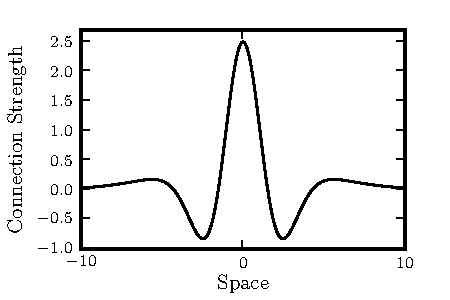
\includegraphics{./Graph/Cross_section_kernel.pdf} 
   	\end{center}
   	\caption{A Mexican-hat connectivity kernel, $w(\mathbf{r},\mathbf{r'})$, used in this paper. The function $w(.)$ is rotationally symmetric (isotropic) about zero, hence a cross-section captures the important aspect of the connectivity kernel's shape. The kernel decays asymptotically to zero.} 
   \end{figure}
The firing rate of the presynaptic neurons is related to the postsynaptic membrane potential by the sigmoidal activation function 
\begin{equation}
	\label{ActivationFunction} f\left( v\left( \mathbf{r}', t \right) \right) = \frac{f_{max}}{1 + \exp \left( \varsigma \left( v_0 - v\left(\mathbf{r}',t\right) \right) \right)}. 
\end{equation}
The parameters $f_{max}$ and $v_0$ describe the maximum firing rate and firing threshold of the neural populations. The parameter $\varsigma$ governs the slope of the sigmoid. By substituting equation~\ref{RateBasedInteractions} into \ref{SpikesToPotential} we get the spatiotemporal model 
\begin{equation}
	\label{FullDoubleIntModel} v\left(\mathbf{r},t\right) =
	\int_{-\infty}^t 
	h\left(t - t'\right) \int_\Omega
	w\left(\mathbf{r},\mathbf{r}'\right) 
	f\left( v\left( \mathbf{r}',t \right)\right)
	d\mathbf{r}'dt'.
\end{equation}
To arrive at the final form of the model, we shall express the synaptic response kernel as a Green's function 
\begin{equation}
	\label{GreensFuncDef} Dh\left( t \right) = \delta \left( t \right), 
\end{equation}
where $D=\frac{d}{dt} + \zeta$ is a temporal differential operator and $\delta(t)$ is the Dirac-delta function giving 
\begin{equation}
	\label{FinalFormContinuous} 
	\frac{dv\left( \mathbf{r},t \right)}{dt} + \zeta v\left( \mathbf{r},t \right) = \int_\Omega {w\left( \mathbf{r},\mathbf{r}' \right)f\left( {v\left( \mathbf{r}',t \right)} \right)d\mathbf{r}'}. 
\end{equation}
To arrive at the integro-difference equation (IDE) form of the model, we discretise time using a first-order Euler method (see~\ref{Time Discretization}) giving 
\begin{equation}
	\label{DiscreteTimeModel} 
	v_{t+T_s}\left(\mathbf{r}\right) = 
	\xi v_t\left(\mathbf{r}\right) + 
	T_s \int_\Omega { 
	    w\left(\mathbf{r},\mathbf{r}'\right)
	    f\left(v_t\left(\mathbf{r}'\right)\right) 
	d\mathbf{r}'} 
	+ e_t\left(\mathbf{r}\right), 
\end{equation}
where $T_s$ is the time step, $\xi = 1-\zeta T_s$ and $e_t(\mathbf{r})$ is an $i.i.d.$ disturbance such that $e_t\sim\mathcal{GP}(\mathbf 0,\gamma(\mathbf{r}-\mathbf{r}'))$. Here $\mathcal{GP}(\mathbf 0,\gamma(\mathbf{r}-\mathbf{r}'))$ denotes a spatial Gaussian Process with mean zero and covariance function $\gamma(\mathbf{r}-\mathbf{r}')$~\cite{Rasmussen2005}. This term is added to account for uncertainty in the model. To simplify the notation, the index of the future time sample, $t+T_s$, shall be referred to as $t+1$ throughout the rest of the paper. 

The mapping between the membrane voltage and the collected iEEG/LFP data is modelled using the observation function 
\begin{equation}
    \label{eq:ObservationEquation}
	\mathbf{y}_t =
	\int_{\Omega}{
	    m\left(\mathbf{r}_n-\mathbf{r}'\right)v_t\left(\mathbf{r}'\right)
	d\mathbf{r}'} + 
	\boldsymbol{\varepsilon}_t, 
\end{equation}
where $\mathbf{r}_n$ defines the location of the sensors in the field, $n=1,...,N$ indexes the sensors and $\boldsymbol{\varepsilon}_t \sim \mathcal{N}\left(0,\Sigma_{\varepsilon}\right)$, $\mathcal{N}\left(0,\Sigma_{\varepsilon}\right)$ denotes the multivariate normal distribution with mean zero and covariance matrix $\Sigma_{\varepsilon}$. The output kernel $m(\mathbf{r}-\mathbf{r}')$ governs the sensor pick-up geometry where 
\begin{equation}
	m\left(\mathbf{r}-\mathbf{r}'\right) = \exp{\left(-\frac{(\mathbf{r}-\mathbf{r}')^\top(\mathbf{r}-\mathbf{r}')}{\sigma_m^2}\right)}. 
\end{equation}

\subsection{Derivation of Finite Dimensional State-Space Model} 
In order to implement standard estimation techniques, we use a decomposition of the field using a set of Gaussian basis functions that are defined by
\begin{equation}\label{eq:FieldBasisFunction}
	\phi\left(\mathbf{r}-\mathbf{r}'\right) =
\exp{\left(-\frac{(\mathbf{r}-\mathbf{r}')^\top(\mathbf{r}-\mathbf{r}')}{\sigma_{\phi}^2}\right)}. 
\end{equation}
Decomposition allows a continuous field to be represented by a finite-dimensional state vector. This facilitates application of standard nonlinear state estimation methods such as the unscented Kalman filter. The field decomposition is described by 
\begin{equation}
	\label{DefFieldDecomp} v_t\left(\mathbf{r}\right) \approx \boldsymbol{\phi}^{\top}\left(\mathbf{r}\right) \mathbf{x}_t, 
\end{equation}
where $\mathbf{\boldsymbol{\phi}}(\mathbf{r})$ is a vector of Gaussian basis functions that are scaled by the state vector, $\mathbf{x}_t$. %The choice of Gaussian basis functions can be justified by the existence of the so called bump solutions for this class of model, which have a Gaussian shape~\cite{Coombes2005}. 
The width and positioning of the basis functions can be determined by spectral analysis (explained in detail in Section~\ref{SpectralAnalysisSection}). The connectivity kernel can also be decomposed as 
\begin{equation}\label{DefKernelDecomp}
	 w\left(\mathbf{r},\mathbf{r}'\right) =\boldsymbol{\psi}^\top\left(\mathbf{r},\mathbf{r}'\right) \boldsymbol{\theta},
\end{equation}
where $\boldsymbol{\psi}(r,r')$ is a vector of Gaussian basis functions and $\boldsymbol{\theta}$ is a vector of scaling parameters. By assuming a Gaussian isotropic connectivity structure, the kernel basis functions can be written as $\psi(\mathbf{r}-\mathbf{r}')$. We will assume that we know the parametric form of the connectivity basis functions, where the scaling parameters $\boldsymbol{\theta}$ are unknown. Each connectivity basis function can, individually, be considered a layer in the Wilson and Cowan model, representing short range excitation, surround inhibition and mid-range excitation. Making substitutions of equations~\ref{DefFieldDecomp} and~\ref{DefKernelDecomp} into~\ref{DiscreteTimeModel} we get 
\begin{equation}
	\label{reduced continuous model}\boldsymbol{\phi}^{\top}(\mathbf{r})\mathbf{x}_{t+1}= T_s\int_\Omega{f(\boldsymbol{\phi}^{\top}(\mathbf{r}')\mathbf{x}_t )\boldsymbol{\psi}^{\top}(\mathbf{r}-\mathbf{r}')d\mathbf{r}'}\boldsymbol{\theta}
	+ \xi\boldsymbol{\phi}^{\top}(\mathbf{r})x_t + e_t(\mathbf{r}). 
\end{equation}
Next we multiply equation~\ref{reduced continuous model} by $\boldsymbol{\phi}(r)$ and integrate over the spatial domain $\Omega$ to get 
\begin{equation}
    \begin{split}
	\label{StartofReduction}
	\lefteqn{ \int_\Omega {\boldsymbol{\phi} \left(\mathbf{r}\right)\boldsymbol{\phi}^{\top}\left(\mathbf{r}\right) d\mathbf{r}} \mathbf{x}_{t+1}=} \\
 &T_s \int_\Omega {\boldsymbol{\phi} (\mathbf{r}) \int_\Omega {\boldsymbol{\psi}^{\top} (\mathbf{r}-\mathbf{r}') f(\boldsymbol{\phi}^{\top}(\mathbf{r}') \mathbf{x}_t ) d\mathbf{r}'}d\mathbf{r}}\boldsymbol{\theta}  \\ & + \xi\int_\Omega {\boldsymbol{\phi}(\mathbf{r})\boldsymbol{\phi}^{\top}(\mathbf{r})d\mathbf{r}} \mathbf{x}_t+
\int_\Omega{\boldsymbol{\phi} (\mathbf{r}) e_t(\mathbf{r})d\mathbf{r}}. 
\end{split}
\end{equation}
Now defining
\begin{equation}\label{eq:DefGamma}
	\boldsymbol{\Gamma} \triangleq \int_\Omega {\boldsymbol{\phi} \left(\mathbf{r}\right)\boldsymbol{\phi} ^{\top}\left(\mathbf{r}\right)d\mathbf{r}}, 
\end{equation}
and substituting this into equation~\ref{StartofReduction} and cross-multiplying by $\boldsymbol{\Gamma}^{-1}$ gives 
\begin{equation}
    \label{eq:ReducedForm}
    \begin{split}
	 \mathbf{x}_{t+1} = T_s\boldsymbol{\Gamma}^{-1}
	 \int_\Omega \boldsymbol{\phi}(\mathbf{r}) 
	 \int_\Omega \boldsymbol{\psi}^{\top} (\mathbf{r}-\mathbf{r}')f(\boldsymbol{\phi}^{\top}(\mathbf{r}')\mathbf{x}_t) d\mathbf{r}' d\mathbf{r} \boldsymbol{\theta} \\ 
	 + \xi\mathbf{x}_t + \boldsymbol{\Gamma}^{-1} \int_\Omega{\boldsymbol{\phi}(\mathbf{r}) e_t(\mathbf{r})d\mathbf{r}}.
	 \end{split}
\end{equation}
This can be simplified by exploiting the symmetry (isotropy) of the connectivity kernel where
\begin{equation}
	\boldsymbol{\psi} (\mathbf{r}-\mathbf{r}') = \boldsymbol{\psi} (\mathbf{r}'-\mathbf{r}).
\end{equation}
To make the simplification, we first define
\begin{equation}\label{eq:DefPsi}
	\boldsymbol{\Psi}(\mathbf{r}') \triangleq T_s\boldsymbol{\Gamma}^{-1}\int_\Omega {\boldsymbol{\phi}(\mathbf{r})\boldsymbol{\psi}^{\top} (\mathbf{r}'-\mathbf{r})d\mathbf{r}},
\end{equation}
which is constant and can be defined analytically. Now substituting equation~\ref{eq:DefPsi} into~\ref{eq:ReducedForm} gives
\begin{eqnarray}
	\mathbf{x}_{t+1} = \int_\Omega \boldsymbol{\Psi}(\mathbf{r}') f(\boldsymbol{\phi}^{\top}(\mathbf{r}')\mathbf{x}_t) d\mathbf{r}' \boldsymbol{\theta} + \xi\mathbf{x}_t\nonumber \\
+ \boldsymbol{\Gamma}^{-1} \int_\Omega{\boldsymbol{\phi}(\mathbf{r})e_t(\mathbf{r})d\mathbf{r}}.
\end{eqnarray}
Now we define the state disturbance as
\begin{equation}\label{eq:AppendixWt} 
	\mathbf{e}_t \triangleq \boldsymbol{\Gamma}^{-1}\int_\Omega {\boldsymbol{\phi} ( \mathbf{r} )e_t( \mathbf{r} )d\mathbf{r}} 
\end{equation}
which is a zero mean normally distributed white noise process with covariance (see~\ref{ColoredNoise})
\begin{equation}
	\boldsymbol\Sigma_e =\mathbf{\Gamma}^{-1}\int_{\Omega}\int_{\Omega}\boldsymbol{\phi}\left(\mathbf r\right) \gamma\left(\mathbf r- \mathbf r' \right)\boldsymbol{\phi}\left(\mathbf r'\right)^{\top}d\mathbf r' d\mathbf r\mathbf{\Gamma}^{- \top}. 
\end{equation}
Under the assumption that the basis function decomposition is accurate, the observation equation of the reduced model is found by substituting equation~\ref{DefFieldDecomp} into~\ref{eq:ObservationEquation} giving
\begin{equation}\label{eq:ReducedObservationEquation}
	\mathbf{y}_t = \int_{\Omega}{m\left(\mathbf{r}_n-\mathbf{r}'\right)\boldsymbol{\phi}^{\top}\left(\mathbf{r}\right) \mathbf{x}_td\mathbf{r}'} + \boldsymbol{\varepsilon}_t. 
\end{equation}
The observation equation is linear and can be written in the more compact form
\begin{equation}\label{ObservationEquation} 
	\mathbf{y}_t = \mathbf{C}\mathbf{x}_t + \boldsymbol{\varepsilon}_t,
\end{equation}
where the observation matrix is 
\begin{equation}
	\mathbf{C} = \left[
	\begin{array}{{ccc}} 
		c_{1,1} & \dots & c_{1,L} \\
		\vdots & \ddots & \vdots \\
		c_{N,1} & \dots & c_{N,L} 
	\end{array}
	\right] 
\end{equation}
where $L$ is the number of basis functions used to decompose the neural field and 
\begin{equation}
	c_{i,j} = \int_{\Omega}m(\mathbf{r}_i - \mathbf{r}')\boldsymbol{\phi}_j(\mathbf{r}')d\mathbf{r}'. 
\end{equation}
Now we have the final form of the state-space model where
\begin{equation}\label{eq:finalformstatespacemodel}
	\mathbf{x}_{t+1} = Q(\mathbf{x}_t) +\mathbf{e}_t.
\end{equation}
\begin{equation} 
	\mathbf{y}_t = \mathbf{C}\mathbf{x}_t + \boldsymbol{\varepsilon}_t
\end{equation}
and 
\begin{equation}\label{eq:QmatrixForSigmapoints}
	Q(\mathbf{x}_t) = \int_\Omega \boldsymbol{\Psi}(\mathbf{r}') f(\boldsymbol{\phi}^{\top}(\mathbf{r}')\mathbf{x}_t) d\mathbf{r}' \boldsymbol{\theta} + \xi\mathbf{x}_t.
\end{equation}

% \begin{equation}
% \mathbf{C} = \left[\begin{array}{{cccc}}
% \int_{\Omega}m(\mathbf{r}_1 - \mathbf{r}')\boldsymbol{\phi}_1(\mathbf{r}')d\mathbf{r}' & \int_{\Omega} m(\mathbf{r}_1 - \mathbf r')\boldsymbol \phi_2(\mathbf r')d\mathbf r' & \dots
% &\int_{\Omega}m(\mathbf r_1 - \mathbf r')\boldsymbol \phi_n(\mathbf
% r')d\mathbf r' \\
% \int_{\Omega}m(\mathbf r_2 - \mathbf r')\boldsymbol \phi_1(\mathbf
% r')d\mathbf r'&\int_{\Omega}m(\mathbf r_2 - \mathbf r')\boldsymbol
% \phi_2(\mathbf r')d\mathbf r'& \dots &\int_{\Omega}m(\mathbf r_2 -
% \mathbf r')\boldsymbol \phi_n(\mathbf r')d\mathbf r'\\
% \vdots&\vdots&\ddots&\vdots\\
% \int_{\Omega}m(\mathbf r_{n_y} - \mathbf r')\boldsymbol \phi_1(\mathbf
% r')d\mathbf r'&\int_{\Omega}m(\mathbf r_{n_y} - \mathbf r')\boldsymbol
% \phi_2(\mathbf r')d\mathbf r'& \dots &\int_{\Omega}m(\mathbf r_{n_y} -
% \mathbf r')\boldsymbol \phi_n(\mathbf r')d\mathbf r'
% \end{array}\right],
% \end{equation}
% and $m(\mathbf r_n - \mathbf{r}')$ is the observation kernel.
\section{Spectral Analysis and Model Selection}\label{SpectralAnalysisSection} Spectral analysis has been used to identify both the number of sensors and the number of basis functions required to reconstruct the neural field from sampled observations \cite{Sanner1992,Scerri2009}. Based on a two-dimensional extension of Shannon's sampling theorem \cite{Peterson1962}, the spatial bandwidth of the observed field can be used to provide a lower bound on both the number of sensors and the number of basis functions required to capture the dominant spectral characteristics of the neural field.

Let the spectral representation of the post-synaptic membrane voltage field at time $t$ be denoted by $V_t(\boldsymbol{\nu})$. According to Shannon's sampling theorem, the field must be spatially band-limited for an accurate reconstruction using spatially discrete observations. Nevertheless, an approximate reconstruction can be obtained if the field is approximately band-limited with 
\begin{equation}
	V_t(\boldsymbol{\nu}) \approx 0 ~ \forall \boldsymbol{\nu} > \boldsymbol{\nu}_c,
\end{equation}
where $\boldsymbol{\nu}_c$ is a cutoff frequency (typically taken as the -3~dB point) with $\boldsymbol{\nu}_c = [\nu_c ~ \nu_c]^\top$. Given such a band-limited field, the distance between adjacent sensors, $\Delta_y$, must satisfy 
\begin{equation}
	\label{eq:MinimumSensorDistance} \Delta_y < \frac{1}{2\rho_y\nu_{c}}, 
\end{equation}
where $\rho_y \in \mathbb{R} \ge 1$ is an oversampling parameter. This condition must be satisfied to avoid spatial spectral aliasing effects when reconstructing the hidden dynamic field, $v_t(\mathbf{r})$, using the sampled observations, $\mathbf{y}_t$.

In practice, it is difficult to estimate the bandwidth of the cortex using traditional electrophysiological measurements, possibly preventing us from positioning sensors in accordance to equation~\ref{eq:MinimumSensorDistance}. However, we envisage it may be possible to estimate the spatial bandwidth using other modalities with higher spatial resolution such as, fMRI, NIRS or other optical imaging techniques~\cite{Issa2000}. Nevertheless, spectral aliasing can still be avoided by a proper choice of the spatial sampling distance given the sensors' spectral characteristics. The spatial extent of the sensors results in a spectral low-pass action, thus providing spatial anti-aliasing filtering. Such sensors therefore can only sense the field up to a known spatial bandwidth, denoted by $\nu_{cy}$. Aliasing can then be avoided by positioning the sensors according to equation~\ref{eq:MinimumSensorDistance}, with $\nu_{cy}$ replacing $\nu_c$. 

Although such sensors avoid errors due to aliasing, they attenuate the high spatial frequency variations in the observations. Therefore, any procedure applied to estimate the original field or the underlying connectivity structure from these band-limited observations has the potential to underestimate the high spatial frequency components of both the field and the connectivity kernel. This motivates the use of sensors with wider bandwidths (narrower in space). Nevertheless, this choice would require more sensors in order to satisfy Shannon's sampling theorem for a reasonable spatial region. Therefore, a compromise needs to be found between the bandwidth of the sensor response, the accuracy of the estimation results, the number of sensors used and the computational demands of the estimation procedure when designing experiments.

Similar considerations need to be made regarding the representation of the dynamic field, $v_t(\mathbf{r})$, using the basis function decomposition. Again applying Shannon's sampling theorem, the minimum distance between basis functions must satisfy 
\begin{equation}\label{eq:BasisFunctionSeparation}
	\Delta_{\phi} < \frac{1}{2\rho_{\phi}\nu_{cy}}
\end{equation}
where $\rho_{\phi} \in \mathbb{R} \ge 1$ is an oversampling parameter to determine the basis function separation. 

The field basis function widths can also be inferred using spectral considerations~\cite{Sanner1992,Scerri2009}. To demonstrate this, we begin with the two-dimensional Gaussian basis function defined as
\begin{equation}
 \phi(\mathbf r)=\mathrm{exp}\left({-\frac{1}{\sigma_{\phi}^2} \mathbf r^\top\mathbf r}\right)
\end{equation}
with the corresponding Fourier transform
\begin{equation}\label{eq:GaussianFT}
\boldsymbol\Phi(\boldsymbol \nu)=\left(\frac{1}{\pi\sigma_{\nu}^2}\right)\mathrm{exp}\left(-\frac{1}{\sigma_{\nu}^2}\boldsymbol\nu^\top \boldsymbol\nu\right),
\end{equation}
where 
\begin{equation}\label{eq:GaussianFTWidth}
	\sigma^2_{\nu} = \frac{1}{\pi^2\sigma_{\phi}^2}. 
\end{equation}
To obtain a 3~dB attenuation at $\boldsymbol\nu_{cy}$, the basis function width, $\sigma^2_{\phi}$, should be chosen to be
\begin{equation}\label{eq:WidthCutOffRelationship}
 \sigma^2_{\phi}= \frac{1}{\pi^2\sigma_{\nu_{cy}}^2},
\end{equation}
where
\begin{equation}\label{eq:WidthFrequencyRelationship}
 \sigma^2_{\nu_{cy}}= \frac{2\boldsymbol\nu_{cy}^\top \boldsymbol\nu_{cy}}{\ln 2}.
\end{equation}
This ensures that the basis functions can represent the neural field with frequency content up to $\boldsymbol\nu_{cy}$. Derivations for equations~\ref{eq:GaussianFT} and \ref{eq:WidthFrequencyRelationship} are given in~\ref{ap:FrequencyAnalysis}.

Alternatively, given the basis function width, the spatial cut-off frequency of the field modelled by the decomposition can be determined from spectral analysis. This is particularly useful when considering the spatially distributed basis functions, since Shannon's sampling theorem is derived for perfect point sensors. To calculate the cut-off frequency imposed by the basis function, $\boldsymbol{\nu}_{c\phi}$, we rearrange equations~\ref{eq:WidthCutOffRelationship} and \ref{eq:WidthFrequencyRelationship} giving
\begin{equation}\label{eq:CutoffFromBasisFuncWidth}
	\boldsymbol{\nu}_{c\phi}=\sqrt{\frac{\ln(2)}{2\pi^2\sigma_{\phi}^2}}.
\end{equation} 

Note that for a spatially homogeneous isotropic field, the basis functions can be placed on a regular grid. Thus, the knowledge of the distance between basis functions can be used to determine the total number of basis functions required to represent a known spatial region.

% 
% Due to the high dimensionality of the brain and the current electrode systems, we can not expect to have more sensors than basis functions.
\section{State and Parameter Estimation}\label{StateAndParameterEstimationSection} In this section we describe the procedure for estimating the states, $\mathbf{x}_t$, the connectivity kernel parameters, $\boldsymbol \theta$, and the synaptic time constant, $\xi$. The estimation process is a two part iterative algorithm, consisting of a state estimation step followed by a parameter estimation step. At each iteration, the sequence of estimated state vectors is used to update the parameter set. The resulting parameters are then used when estimating the new state vector sequence for the next iteration. The procedure stops when the parameters converge. The algorithm is initialised using a bounded random state vector sequence guaranteeing that the initial estimated parameter set forms a stable kernel.

The unscented Rauch Tung Striebel smoother (URTSS)~\cite{Sarkka2010} is used for the state estimation. The URTSS incorporates an unscented Kalman filter (UKF)~\cite{Julier1997, Merwe2003} in a forward iteration to estimate posterior states, $\hat{\mathbf x}_t^{f}$, followed by a backward iteration to compute the smoothed state estimates, $\hat{\mathbf x}_t^{b}$. The first and the second order moments of the predicted state are captured by propagating the so-called sigma points through the state equation. The sigma points, $\mathcal X_i$, are calculated using the unscented transform as follows:
\begin{equation}\label{eq:sigmapoints1}
	\mathcal X_{0}=\bar x 
\end{equation}
\begin{equation}
	\mathcal X_{i}=\bar x+\left(\sqrt{( L + \lambda)\mathbf P_x}\right)_i, \quad i=1, \dots, L 
\end{equation}
\begin{equation}\label{eq:sigmapoints2}
	\mathcal X_{i}=\bar x-\left(\sqrt{( L + \lambda)\mathbf P_x}\right)_{i- L}, \quad i= L+1, \dots, 2 L 
\end{equation}
where $\bar x$ represents either $\hat{\mathbf x}_t^{f}$ or $\hat{\mathbf x}_t^{b}$, $\mathbf{P}_x$ is the corresponding covariance matrix from the filtering or smoothing, $\left(\sqrt{( L + \lambda)\mathbf P_x}\right)_i$ is the $i^{th}$ column of the weighted matrix square root of $\mathbf P_x$ and $L$ is the dimension of the state space. The total number of sigma points is $2L+1$. The scaling parameter, $\lambda$, is defined as 
\begin{equation}\label{eq:sigmapoints3}
	\lambda=\alpha^2( L+\kappa) - L, 
\end{equation}
where the constant $\alpha$ determines the spread of the sigma points, $\beta$ incorporates prior knowledge of the distribution of $\mathbf{x}$ and $\kappa$ is a scaling parameter (see~\cite{Haykin2001} for more details). 

The sigma vectors are propagated through the system equations and weighted to form the predicted mean and covariance. The weights are calculated by 
\begin{equation}
	\mathbf W_0^{(m)}=\frac{\lambda}{ L+\lambda} 
\end{equation}
\begin{equation}
	\mathbf W_0^{(c)}=\frac{\lambda}{ L+\lambda}+(1-\alpha^2+\beta) 
\end{equation}
\begin{equation}
	\mathbf W_i^{(m)}=\mathbf W_i^{(c)}=\frac{1}{2( L+\lambda)} \quad i=1, \dots, 2L, 
\end{equation}
where the superscripts $m$ and $c$ stand for mean and covariance. Since the observation equation is linear (equation~\ref{ObservationEquation}) the standard Kalman Filter update equations are used to correct the predicted states. The state estimates from forward filtering are used to form a new set of sigma points for the smoother, as described above. To compute the smoother gain, the cross-covariance matrix of the states, $\mathbf M$, needs to be computed. A summary of the URTSS procedure is given in Algorithm~\ref{UKFAlgorithm}. It should be noted that the disturbance, $\mathbf{e}_t$ and the measurement noise, $\boldsymbol{\varepsilon}_t$, are additive. Therefore, the additive form of the URTSS is used, instead of augmenting the state vector with the noise terms with the added benefit of reducing the dimension and the number of sigma points required in the algorithm.
\begin{algorithm}
	\begin{small}
	\caption{The Unscented RTS Smoother}\label{UKFAlgorithm} 
	\begin{algorithmic}[1] 
		\State Forward initialisation 
		\begin{equation*}
		 \hat{\mathbf x}_0, \mathbf P_0 
		\end{equation*}
		\State Forward iteration: for $t \in \left\lbrace 0,\cdots, T\right\rbrace $,
		calculate the sigma points $\mathcal X_{i,t}^f$ using equations \ref{eq:sigmapoints1}-\ref{eq:sigmapoints3} and propagate through equation~\ref{eq:QmatrixForSigmapoints}
% 		\begin{small}
		\begin{equation*}
			\mathcal X_{i,t+1}^{f-}=Q(\mathcal X_{i,t}^f) \quad i=0, \dots, 2L
		\end{equation*}
% 		\end{small}
		calculate the predicted state and the predicted covariance matrix
		\begin{equation*}
			\hat{\mathbf x}_{t+1}^{f-}=\sum_{i=0}^{2L} W_i^{(m)}\mathcal X_{i,t+1}^{f-} 
		\end{equation*}
		\begin{equation*}
			\mathbf P_{t +1}^{f-}=\sum_{i=0}^{2L} W_i^{(c)}(\mathcal X_{i,t+1}^{f-}-\hat{\mathbf x}_{t +1}^{f-})(\mathcal X_{i,t+1}^{f-}-\hat{\mathbf x}_{t +1}^{f-})^\top+\boldsymbol \Sigma_e 
		\end{equation*}
		compute the filter gain, the filtered state and the filtered covariance matrix using the standard Kalman Filter update equations
		\begin{equation*}
			\mathcal K_{t+1}=\mathbf P_{t +1}^{f-}\mathbf C ^\top(\mathbf C \mathbf P_{t +1}^{f-}\mathbf C ^\top+\boldsymbol \Sigma_{\epsilon})^{-1} 
		\end{equation*}
		\begin{equation*}
			\hat{\mathbf x}_{t+1}^{f}=\hat{\mathbf x}_{t+1}^{f-}+\mathcal K_{t+1}(\mathbf y_{t+1}-\mathbf C\hat{\mathbf x}_{t +1}^{f-}) 
		\end{equation*}
		\begin{equation*}
			\mathbf P_{t+1}^f=(\mathbf I - \mathcal K_{t+1}\mathbf C)\mathbf P_{t +1}^{f-} 
		\end{equation*}
		\State Backward initialisation 
		\begin{equation*}
			\mathbf P_T^b= \mathbf P_T^f, \quad \hat{\mathbf x}^b_T= \hat{\mathbf x}^f_T 
		\end{equation*}
		\State Backward iteration: for $t \in \left\lbrace T-1, \cdots, 0 \right\rbrace $ calculate the sigma points $\mathcal X_{i,t}^b$ and propagate them through equation \ref{eq:QmatrixForSigmapoints}
		\begin{equation*}
			\mathcal X_{i,t+1}^{b-}=Q(\mathcal X_{i,t}^b) \quad i=0, \dots, 2L
		\end{equation*}
		 compute the predicted state, the predicted covariance matrix and the cross-covariance matrix
		\begin{equation*}
			\hat{\mathbf x}_{t+1}^{b-}=\sum_{i=0}^{2L} W_i^{(m)}\mathcal X_{i,t+1}^{b-} 
		\end{equation*}
		\begin{equation*}
			\mathbf P_{t +1}^{b-}=\sum_{i=0}^{2L} W_i^{(c)}(\mathcal X_{i,t+1}^{b-}-\hat{\mathbf x}_{t +1}^{b-})(\mathcal X_{i,t+1}^{b-}-\hat{\mathbf x}_{t +1}^{b-})^\top+\boldsymbol \Sigma_e 
		\end{equation*}
		\begin{equation*}
			\mathbf M_{t +1}=\sum_{i=0}^{2L} W_i^{(c)}(\mathcal X_{i,t}^{b-}-\hat{\mathbf x}_{t}^{f})(\mathcal X_{i,t+1}^{b-}-\hat{\mathbf x}_{t+1}^{b-})^\top 
		\end{equation*}
		 Compute the smoother gain, the smoothed state and the smoothed covariance matrix
		\begin{equation*}
			\mathbf S_t=\mathbf M_{t +1}\left[ \mathbf P_{t +1}^{b-}\right] ^{-1} 
		\end{equation*}
		\begin{equation*}
			\hat{\mathbf x}_t^b=\hat{\mathbf x}_t^f+\mathbf S_t\left[\hat{\mathbf x}_{t+1}^{b}-\hat{\mathbf x}_{t+1}^{b-}\right] 
		\end{equation*}
		\begin{equation*}
			\mathbf P_{t}^{b}=\mathbf P_{t}^{f}+\mathbf S_t\left[\mathbf P_{t+1}^{b}-\mathbf P_{t+1}^{b-} \right]\mathbf S_t^\top 
		\end{equation*}
	\end{algorithmic}
\end{small}
\end{algorithm}

Although the system is nonlinear, the parameters of the system are linear with respect to the state. This feature is exploited by our procedure where the parameter estimation uses a least squares (LS) method that minimises the sum of the squared errors (of a predicted state update) with each new state vector sequence estimate. To create the least squares parameter estimator, we first define the $L \times n_{\theta}$ matrix
\begin{equation}
	\mathbf{q}(\mathbf{x}_t) = \int_\Omega \boldsymbol{\Psi}(\mathbf{r}') f(\boldsymbol{\phi}^{\top}(\mathbf{r}')\mathbf{x}_t) d\mathbf{r}'.
\end{equation}
Now given a state estimate sequence from the URTSS, we can write
\begin{eqnarray*}
	\mathbf x_{1} &=& \mathbf{q}(\mathbf x_0) \boldsymbol{\theta}+\xi\mathbf x_0+\mathbf e_0 \\
	\mathbf x_{2} &=& \mathbf{q}(\mathbf x_1) \boldsymbol{\theta}+\xi\mathbf x_1+\mathbf e_1  \\
	&\vdots& \\
	\mathbf x_{T}&=&\mathbf{q}(\mathbf x_{T-1}) \boldsymbol{\theta}+\xi\mathbf x_{T-1}+\mathbf e_{T-1}. 
\end{eqnarray*}
This can be written in the compact form
\begin{equation}
	\mathbf Z=\mathbf X \mathbf W+\mathbf{e}, 
\end{equation}
where
\begin{small}
\begin{equation*}
	\mathbf Z=\left[
	\begin{array}{cccc}
		\mathbf x_{1}\\
		\mathbf x_{2}\\
		\vdots\\
		\mathbf x_{T}
	\end{array}
	\right],\quad \mathbf X=\left[
	\begin{array}{cccc}
		\mathbf q(\mathbf x_0)& \mathbf x_{0}\\
		\mathbf q(\mathbf x_1)& \mathbf x_{1}\\
		\vdots & \vdots\\
		\mathbf q(\mathbf x_{T-1})& \mathbf x_{T-1}
	\end{array}
	\right] 
\end{equation*}
\end{small}
and
\begin{small}
\begin{equation*}
\quad \mathbf W=\left[
	\begin{array}{cc}
		\boldsymbol{\theta} \\
		\xi
	\end{array}
	\right],\quad \mathbf{e}=\left[
	\begin{array}{cccc}
		\mathbf e_0\\
		\mathbf e_1\\
		\vdots\\
		\mathbf e_{T-1}
	\end{array}
	\right].
\end{equation*}
\end{small}
Following this, the LS parameter estimates, $ \mathbf{\hat{W}}$, are
\begin{equation}
	\mathbf{\hat{W}}=(\mathbf X^\top\mathbf X)^{-1}\mathbf X^\top\mathbf Z. 
\end{equation}
% The accuracy of the approximation is linked to the time step used in the temporal discretisation of the system, where the state transition appears more linear with a finer resolution. 
% Alternatives to the UKF are the Extended Kalman Filter (EKF)~\cite{Haykin2001} and the Sequential Monte Carlo (SMC) filter~\cite{doucet2001}. The EKF approximates the state transition equation by linearising about the current state estimates (by calculating the Jacobian) at each time instance. The linearisation maintains the Gaussianality of the model. The unscented Kalman filter approximates the posterior state density by a Gaussian distribution using a minimal set of carefully chosen sigma points, while maintaining the nonlinearity in the system. This has been shown to give superior performance over the EKF in state estimation, since the EKF maintains a first order approximation where the UKF provides an approximation accurate at least to the second order. In addition, the computation of the Jacobian used in the EKF can be problematic. SMC filtering can theoretically provide an exact posterior state density for nonlinear systems. However, currently this method is not appropriate for our problem, due to high computation demands. 

%The method is appropriate for state estimation of stochastic nonlinear dynamical systems. 
\section{Results}\label{ResultsSection} The full neural field model derived in Section~\ref{NeuralModelSection} was used to generate the data for state and parameter estimation. All parameters for the model are given in Table~\ref{tab:Model Parameters}. Note that, the parameters for the spatial and temporal aspects of the model can be considered arbitrary when demonstrating the estimation methodology. This is due to the fact that the temporal aspects scale with the sampling rate and the length of the times series, and the spatial aspects scale with the size of the neural field and the space step used for numerical simulation. Figure~\ref{fig:experimental design}(a) shows example data from the sensors of the model and Figure~\ref{fig:experimental design}(b) shows the power spectral density (PSD) of the simulated time-series. The PSD shows the typical $1/f^2$ characteristics of intracranial EEG.
\begin{table}\footnotesize
\centering
\begin{tabular}{ccl}
	\hline\hline Symbol & Value & Units \\
	\hline\hline
	$\tau$ & 0.01 & s$^{-1}$\\
	$f_{max}$ & 10 & spikes/s \\
	$\varsigma$ & 0.8 & spike/mV\\
	$v_0$ & 2 & mV\\
	$\boldsymbol{\theta}$ & $\left[\begin{array}{ccc}
	10 &-8 &0.5
	\end{array}
	\right]^{\top}$ & mV/spike\\
	$\sigma_{\psi_{1}}, \sigma_{\psi_{2}}, \sigma_{\psi_{3}}$ & 1.8, 2.4, 6 & mm\\
	$\sigma_{m},\Delta_{y}$&0.9, 1.5&mm\\
	$\Sigma_{\epsilon}$ &$0.1 \times I_{N} $& mm$^2$ \\
	$\sigma_{\gamma}$&1.3&mm\\
	$\Delta$ & 0.5 & mm \\
	$T_s$ & 1 & ms \\ 
\end{tabular}
\caption{Parameters for the neural field model that are used to generate synthetic data.}
\label{tab:Model Parameters}
\end{table}

The sensors were spaced on a regular square 14 $\times$ 14 grid, the sensor width parameter $\sigma^2_m$ was $0.81$, which provides a width of $1.5$~mm at half the maximum amplitude of the basis function, with spacing $\Delta_y=1.5$~mm. This arrangement modelled the recording as having some cross talk, which is typical for neurophysiological recordings. 
\begin{figure}
   	\begin{center}
    		\subfigure[][]{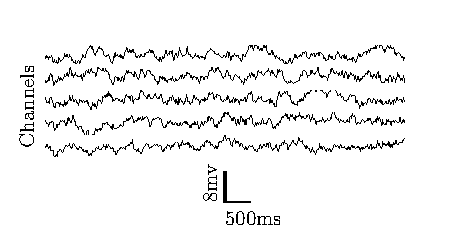
\includegraphics{./Graph/ExperimentFigureEEGPy.pdf}} \\
   		\subfigure[][]{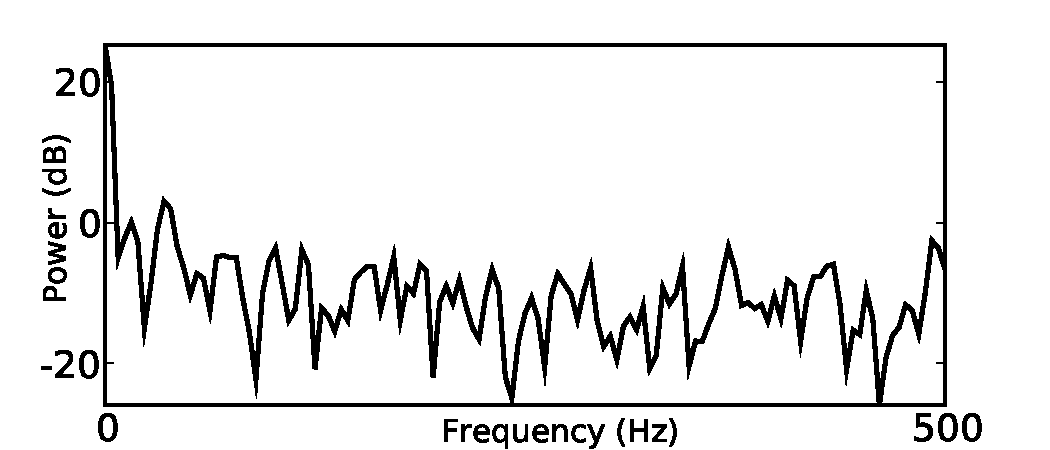
\includegraphics{./Graph/ExperimentFigurePSDPy.pdf}} \\
   	\end{center}
   	\caption{\textbf{a.} Example of data generated by the full neural field model from the first 5 sensors. \textbf{b.} Power spectral density of the data generated by an observation showing the typical $1/f^2$ characteristic of intracranial EEG.} 
\label{fig:experimental design}
\end{figure}
\subsection{Spatial Frequency Analysis} 
Using the model selection techniques described in Section~\ref{SpectralAnalysisSection}, the spatial frequency analysis was used to confirm that the spacing and width of the sensors was adequate to capture the significant dynamics of the field. Figure~\ref{fig:FieldFFT} shows the spatial frequency of the neural field. The cut-off frequency of the neural was taken to be $\nu_c \approx 0.24$~Hz ($-3$~dB point). From equation~\ref{eq:MinimumSensorDistance}, this yielded a minimum sensor separation of $2.05$~mm. This confirms that the separation of $\Delta_{y} = 1.5$~mm was sufficient to prevent problems associated with spatial aliasing.
\begin{figure}
\centering
\subfigure[][]{\label{fig:FieldFFT}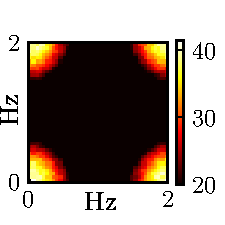
\includegraphics{./Graph/FFTTrueField.pdf}}
\subfigure[][]{\label{fig:EstimatedFieldFFT}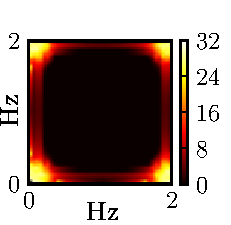
\includegraphics{./Graph/FFTEstimatedField.pdf}}\\
\caption{Spatial frequency analysis of the neural field. \textbf{a.} The average (over time) power in dB of the spatial frequency of the neural field. \textbf{b.} The average (over time) power in dB of the spatial frequency of the reconstructed neural field from the basis function decomposition. The reconstructed field shows a narrower bandwidth as a result of the band limiting properties of the sensors and basis functions.}
\label{fig:FFTTrueEstimate}
\end{figure}

The spatial frequency of the observed field is shown in Figure~\ref{fig:ObservationFreqAnal}. The cut-off frequency was taken to be $\nu_{cy} \approx 0.19$~Hz ($-3$~dB point) \dean{the Figure~\ref{fig:SensorFunctionFreqResponse} has the cut-off as $\approx 0.2$~Hz!}. The observation cut-off frequency is lower than the field cut-off due to the low-pass filtering effect of the sensors. The spatial frequency response of the sensors can be seen in Figure~\ref{fig:SensorFunctionFreqResponse}. Using an oversampling parameter of $\rho_{\phi}=1$, the minimum distance between basis functions was calculated to be $2.63$~mm to satisfy Shannon's sampling criterion (from equation~\ref{eq:BasisFunctionSeparation}). The distance between basis functions, $\Delta_{\phi}$, was set to $2.5$~mm, which is sufficient to capture the significant dynamics according to our criteria.

Given the basis function separation, the basis function width parameter was set to $\sigma_{\phi}^2=2.5$~mm. This allowed a smooth representation of the field by the basis function reconstruction up to a spatial frequency $\mathbf{\nu_{c\phi}} \approx 0.12$~Hz, as described by equation~\ref{eq:CutoffFromBasisFuncWidth}. The band-limiting effect is due to the spatial frequency response of the basis functions as seen in Figure~\ref{fig:BasisFunctionFreqResponse}.
\begin{figure} 
	\begin{center}
		\subfigure[][]{\label{fig:ObservationFreqAnal}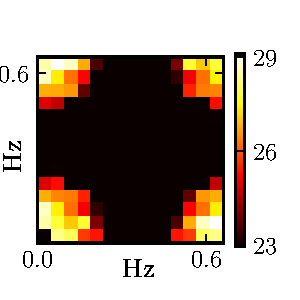
\includegraphics{./Graph/ObservationFrequencyResponse.pdf}}\\	
		\subfigure[][]{\label{fig:SensorFunctionFreqResponse}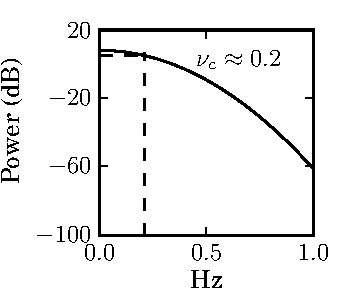
\includegraphics{./Graph/SensorChar.pdf}}
		\subfigure[][]{\label{fig:BasisFunctionFreqResponse}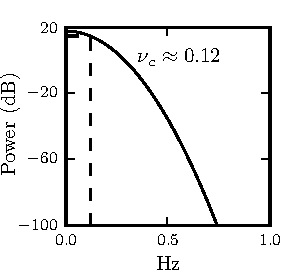
\includegraphics{./Graph/BasisChar.pdf}}
	\end{center}
	\caption{\dean{Can we use $\nu_{cy}$ and $\nu_{c\phi}$ in the labels on the graphs?} Spatial frequency analysis. The dashed line shows the cut-off frequency (-3 dB point). \textbf{a.} Two-dimensional spatial frequency in power dB, averaged over 400 time steps) of the observed field. The symmetry of the sensors and field basis functions allow for the 1-dimensional representation of the spectral characteristics. \textbf{b.} The spatial frequency response of a 1-dimensional model sensor. \textbf{c.} The spatial frequency response of a 1-dimensional neural field basis function, illustrating a narrower band width than the sensors.} 
\end{figure}

\subsection{State and Parameter Estimates} 
\label{sec:state_and_param_results}
To demonstrate the performance of the parameter and state estimation, a Monte Carlo approach was employed where $100$ realisations of the data were generated. Each realisation consisted of $500$~ms of data (sampled at $1$~kHz) and the estimation was applied to the final $400$~ms, allowing the model's initial transients to die out. The initial state and parameters were unknown to the estimator. Eleven iterations of the estimation algorithm were used to ensure the parameters  converge.

The distribution of the estimated parameters is shown in Figure~\ref{fig:Parameters}. The mean parameter estimates and the corresponding standard deviations are given in Table~\ref{tab:Parameters estimates}. The estimates for $\xi$, where $\xi=1-\zeta T_s $ and $\zeta$ is the reciprocal of the synaptic time constant, are close to the actual values, however show a small bias (with a mean bias of 2.5~\%). The estimates of the connectivity kernel parameters ($\theta_0$, $\theta_1$, $\theta_2$) form distributions that are approximately Gaussian. The mean parameter estimates are in good accordance with the actual values, with biases of 2.778, 7.138 and 10.2~\% for $\theta_0$, $\theta_1$ and $\theta_2$ respectively. The ratios of the estimates ($\hat\theta_0/\hat\theta_1$ and $\hat\theta_0/\hat\theta_2$) are shown in Figure~\ref{fig:ParametersRatio}. The distribution of estimates for $\hat\theta_0/\hat\theta_1$ are relativity tighter\parham{(it's 0.0812 (a bit tighter) and 3.757 respectively)}, though indicate a bias... This indicates the balance of excitation and inhibition can be estimated more accurately than the individual parameters. 

\begin{table}
\centering
\begin{tabular}{cccc}
	\hline\hline Parameter & Actual Value & Mean Estimate $\pm$ Standard Deviation \\
	\hline\hline
 	$\xi$ & 0.9 & 0.925 $\pm$ 0.004 \\
	$\theta_0$ & 10 & 10.295 $\pm$ 2.879 \\
	$\theta_1$ & -8 & -8.571 $\pm$ 1.996 \\
	$\theta_2$ & 0.5 & 0.551 $\pm$ 0.083 \\
\end{tabular}
\caption{Actual parameter values and mean parameter estimates and standard deviation.}
\label{tab:Parameters estimates}
\end{table}

The reconstructed connectivity kernel from the estimated parameters can be seen in Figure~\ref{fig:KernelEstimates}. This Figure verifies the expected net shape of the estimated connectivity kernel is in good accordance to the true kernel. The shape is generally well preserved.

Figure~\ref{fig:ParametersConvergence} shows the rate of convergence for parameter estimates.
\begin{figure}
    \centering
    \subfigure[][]{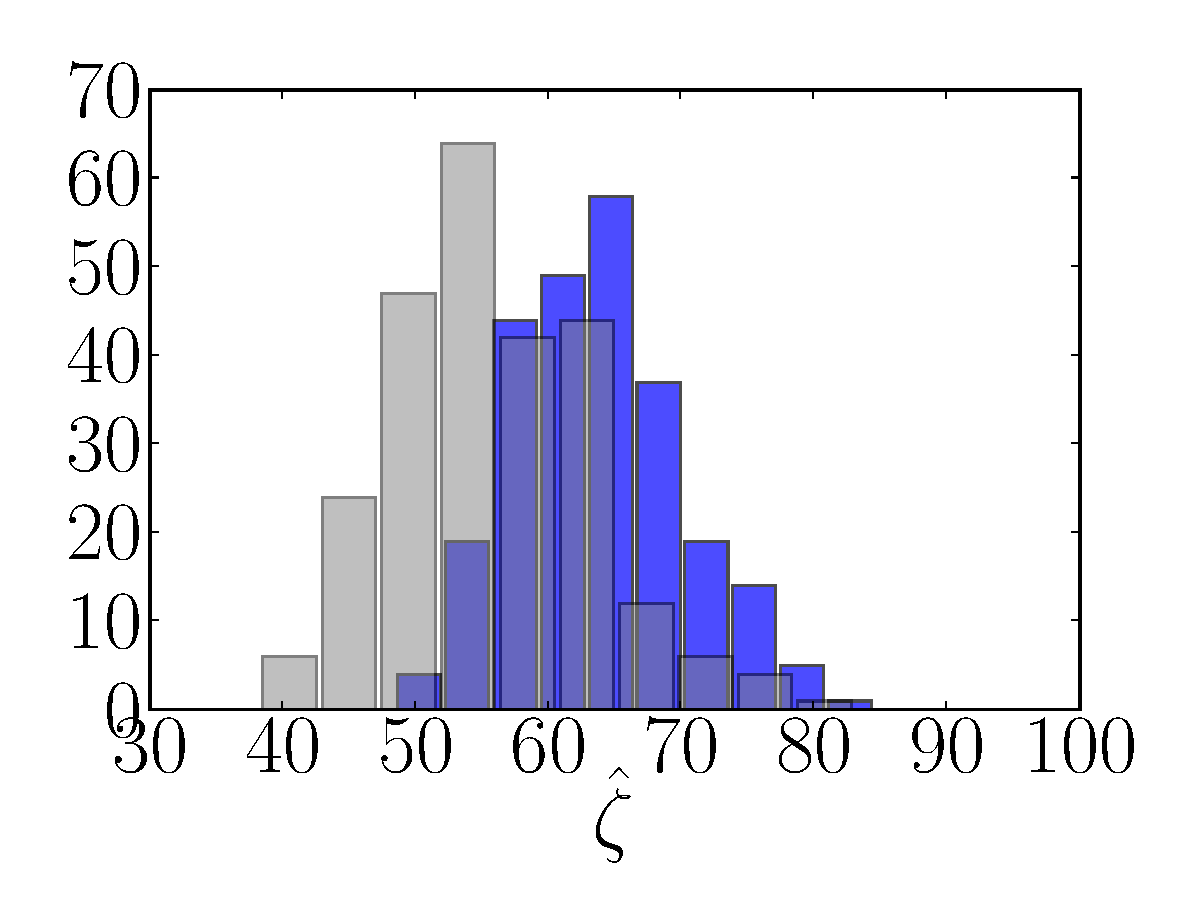
\includegraphics{./Graph/zeta.pdf}}
    \subfigure[][]{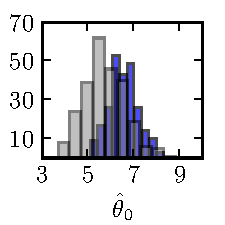
\includegraphics{./Graph/theta0.pdf}}\\
    \subfigure[][]{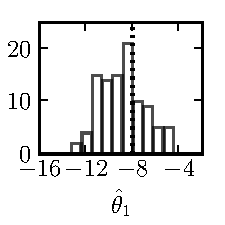
\includegraphics{./Graph/theta1.pdf}}
    \subfigure[][]{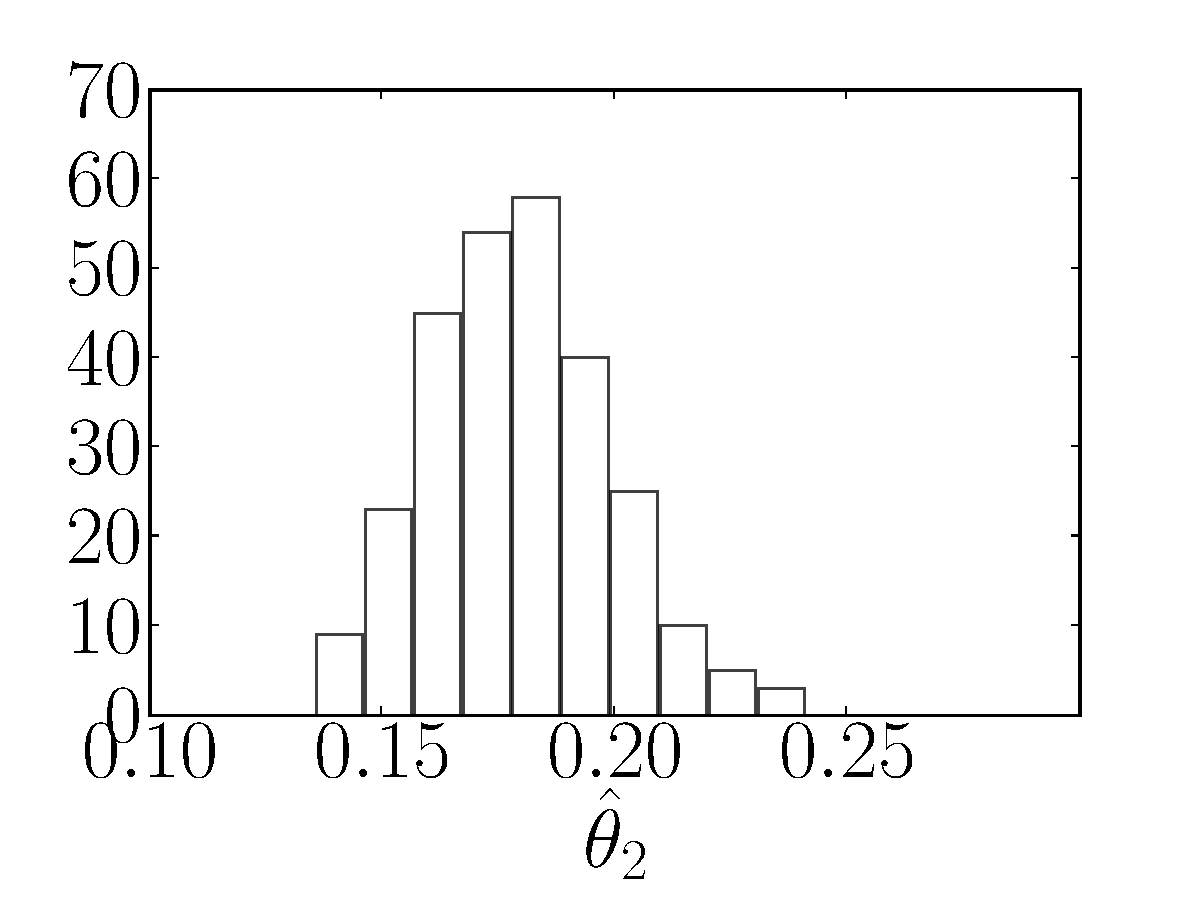
\includegraphics{./Graph/theta2.pdf}}
\caption{Distribution of the parameter estimates over 100
realisations. The dotted line shows the location of the true parameter in each case. \textbf{a.} The distribution of $\xi$ estimates where $\xi=1-\zeta T_s $ and $\zeta$ is the synaptic time constant (true parameter: $\xi=0.9$). \textbf{b.} The distribution of the central excitatory connectivity kernel basis function parameter estimates (true parameter: $\theta_0 = 10$). \textbf{c.} The distribution of the surround inhibition connectivity kernel basis function parameter estimates (true parameter: $\theta_1 = -8$). \textbf{d.} The distribution of the longer range excitatory connectivity kernel basis function parameter estimates (true parameter $\theta_3 = 0.5$).}
\label{fig:Parameters}
\end{figure}
\begin{figure}
    \centering
\subfigure[][]{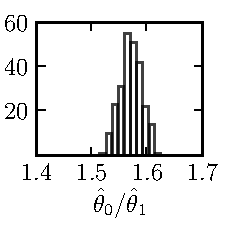
\includegraphics{./Graph/theta0_theta1_ratio.pdf}}
\subfigure[][]{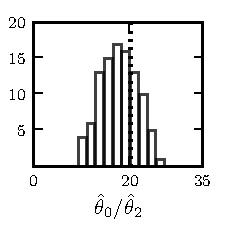
\includegraphics{./Graph/theta0_theta2_ratio.pdf}}\\
\caption{Distribution of the connectivity kernel basis function parameter ratios over 100 realisations. \textbf{a.} The absolute value of the ratio of the local excitatory parameter to the surround inhibition parameter (true ratio is 1.25). \textbf{b.} The ratio of the local excitatory parameter to the longer range excitatory parameter (true ratio is 20). The dotted line shows the location of the true ratio in each case.}
\label{fig:ParametersRatio}
\end{figure}
\begin{figure}
    \centering
\subfigure[][]{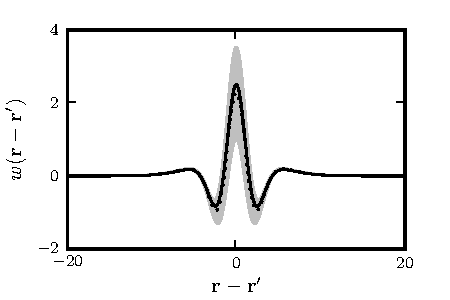
\includegraphics{./Graph/KernelEstimate.pdf}}
\subfigure[][]{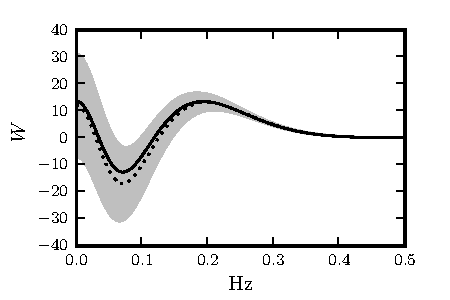
\includegraphics{./Graph/KernelEstimateFFT.pdf}}\\
\caption{Results for connectivity kernel estimate. In all the subplots the true kernel is shown by the solid line, the mean kernel estimate (over 100 realisations) is shown by the dotted line and the 95~\% confidence interval is shown by the shaded grey region. \textbf{a.} Comparison of kernel estimates to true kernel in the spatial domain. \textbf{b.} Comparison of the true kernel to the estimated kernel in the frequency domain.}
\label{fig:KernelEstimates}
\end{figure}
\begin{figure}
        \centering
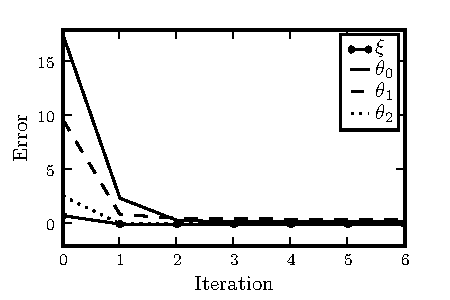
\includegraphics{./Graph/convergence.pdf}
\caption{The mean of the absolute error between true and estimated parameters averaged over 100 runs. All parameters converge after six iterations. The mean difference between errors in consecutive iterations falls below $10^{-4}$ after 6 iterations. }
\label{fig:ParametersConvergence}
\end{figure}

The accuracy for state estimates were evaluated by comparing the field reconstruction (see equation~\ref{DefFieldDecomp}) to the true field using the mean (over time) of the root mean square error (MRMSE) (over space) and standard deviation of the RMSE. The RMSE of the field estimates over time for 100 realisations is shown in Figure~\ref{fig:RMSE}. A snapshot of the true field, the estimated field and their corresponding error is illustrated in Figure~\ref{fig:FieldEstimate}. This figure highlights the loss of the high spatial frequency information in the basis function decomposition.
  \begin{figure}
   	\begin{center}
   		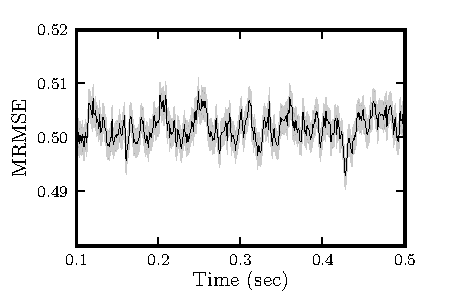
\includegraphics{./Graph/MRMSE.pdf} 
   	\end{center}
   	\caption{The mean of average RMSE of the estimated field over 100 realisations (solid line) and the 95~\% confidence interval (grey region). The error remains consistent over time.} 
\label{fig:RMSE}
   \end{figure}
  
\begin{figure}
\centering 
\subfigure[][]{\label{fig:TrueField}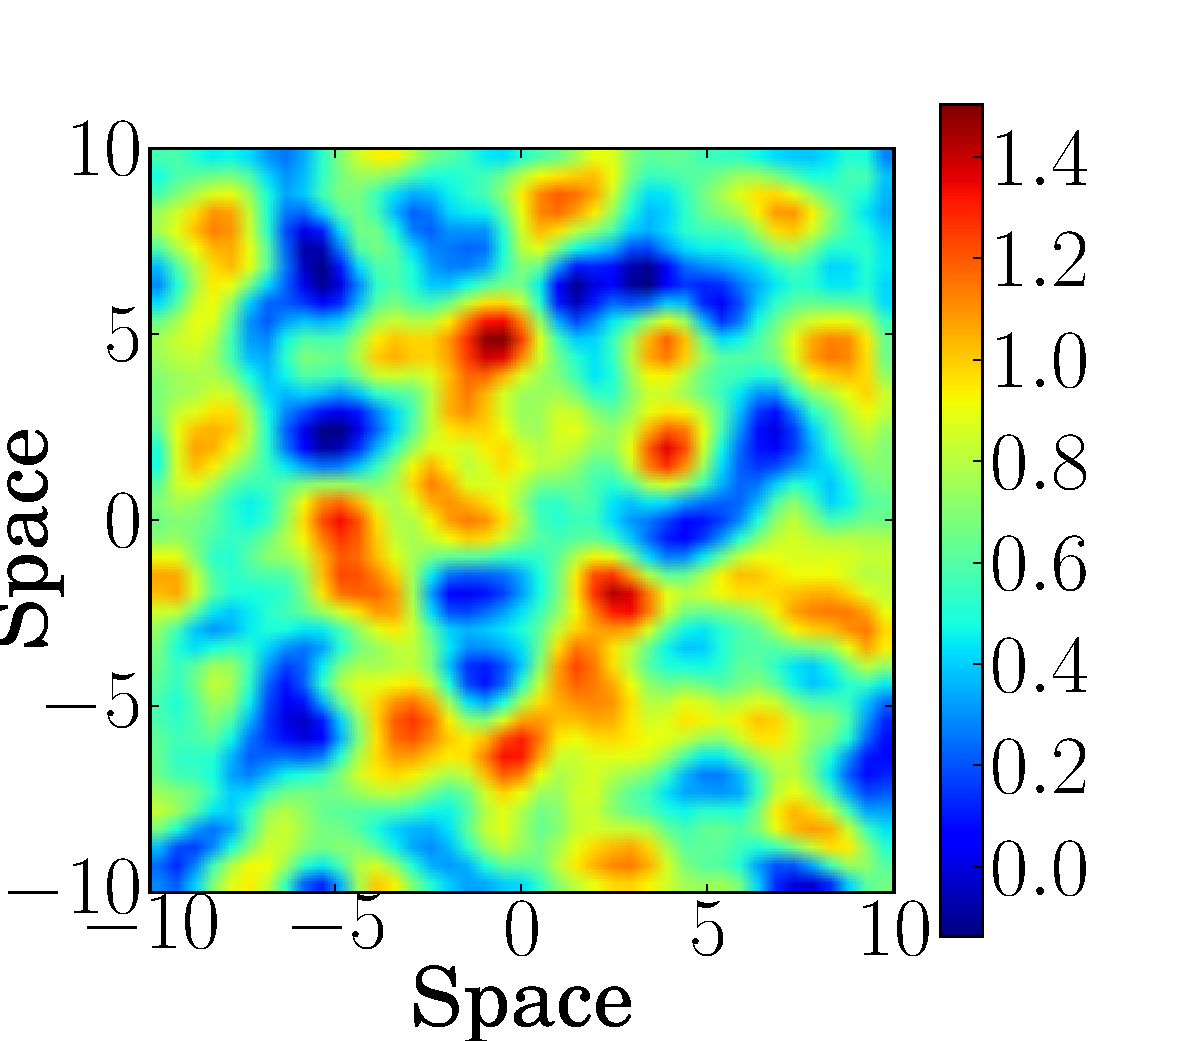
\includegraphics{./Graph/TrueField90.pdf}}
\subfigure[][]{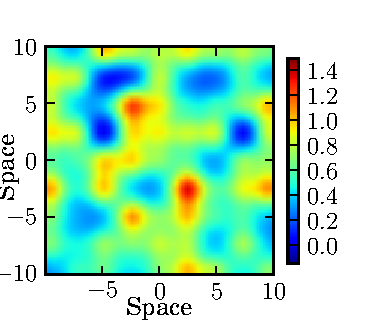
\includegraphics{./Graph/EstimatedField90.pdf}}
\subfigure[][]{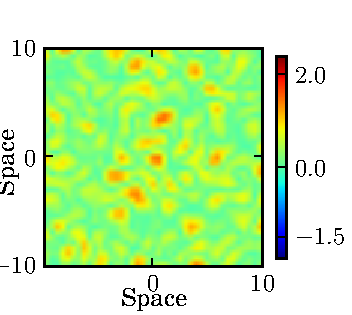
\includegraphics{./Graph/EstimationError90.pdf}}\\
\caption{Examples of the neural fields. \textbf{a.} The true field from the full neural field model which was used to generate data. \textbf{b.} The reconstructed field of the reduced model, showing the effect of the basis function decomposition on the frequency content of the estimated field. \textbf{c.} The absolute error between the true and reconstructed fields, the error shows high frequency behaviour.}
\label{fig:FieldEstimate}
\end{figure}

\section{Discussion}\label{DiscussionSection}

One thing that is shown is that noise has a large impact in the estimation results. To reduce the effect of noise, an evoked response paradigm should be considered when using real data. 

The main contribution of this paper is the methodology for...

To the authors' best knowledge, this is the first paper to propose an estimation framework for intracortical connectivity from electrophysiological data. The importance of the estimation framework can be illustrated by considering that the connectivity structure at this scale can not be estimated using diffusion tensor imaging due to the near isotropic diffusion of water in grey matter~\cite{Assaf2008}. In addition, other non-model-based techniques for estimating functional connectivity, such as Granger causality~\cite{Hesse2003}, the direct transfer function~\cite{Kaminski1991} and partial directed coherence~\cite{Sameshima1999}, are restricted to the spatial scales of the recording electrodes. The model-based technique proposed in this paper estimates the connectivity structure independently of the number of sensors. 

The closest competitor to the integrodifference equation based approach is perhaps the multivariate auto-regressive (MVAR) model. An advantage of the MVAR-based methods is that they allow for anisotropic connectivity, which is present in cortico-cortical fibres. A recent theoretical study~\cite{Jirsa2009} has demonstrated the importance of this multi-scale structure in generating the characteristic rhythms of the brain. A possible method of creating more precise models with this multi-scale structure maybe to estimate anisotropic cortico-cortical connectivity using a MVAR approach and intracortical connectivity using the methods proposed in this paper. 

Generating patient specific neural field models has the potential to have significant impact on several areas of neuroscientific research and clinical neurology. Specifically, the development of a patient-specific state-space model will allow for the application of techniques from engineering to be applied to neuro-dynamics. For example, state tracking could be used in brain-computer interface or epileptic seizure prediction applications, where specific regions of the state-space may indicate intent of movement or imminent seizures. In addition, a patient specific state-space model will allow application of control engineering techniques to robustly prevent the neuro-dynamics entering pathological regions of state-space using electrical stimulation. 

Parameter estimation may also have significant impact on the treatment of disease. For example, recent theoretical work has demonstrated that seemingly similar electrographic seizures in absence epilepsy may arise from either abnormal excitatory or inhibitory mechanisms~\cite{Marten2009}. These very different mechanisms would require very different medications for successful treatment. However, the underlying mechanisms would be hidden from the clinician in the normal clinical setting. Successful parameter estimation has the potential to reveal these hidden mechanisms allowing for improved treatment strategies. 

This estimation framework also has theoretical implications by establishing a framework that has the potential to allow testing of hypotheses that have been generated in theoretical studies and to validate neural field models. For example, it has been hypothesised that so-called ``bump solutions'' are a possible mechanism for short term memory formation~\cite{Coombes2005}. Using the proposed model-based framework, we can reconstruct a neural field from data, and estimate parameters and check if they correspond to the theoretically derived parameters where these bump solutions can exist. In addition, the parameters and the state-space can be explored during other cognitive tasks and states of arousal such as during sleep and anaesthesia. 

\section{Conclusion}
This paper presents a novel framework for state and parameter estimation of spatio-temporal neural fields. A basis function decomposition reduces the infinite dimensional neural field (continuous space) to a finite dimensional state-space model. The level of detail of the estimated field is related to the basis functions decomposition, providing a flexible framework where a trade-off can be made between physiological detail and computational complexity. The effect of the basis function decomposition will restrict the frequency content of the estimated field. This is evident when comparing Figures~\ref{fig:FieldFFT} and~\ref{fig:EstimatedFieldFFT} where the estimated field is spatially band-limited. The spatial frequency content of the field is governed by disturbance covariance and the shape of the connectivity kernel. Using the state-space model, the unscented Rauch Tung Striebel smoother was applied for state estimation. Using the sequence of state estimates, a least squares algorithm was implemented for parameter estimation. We have demonstrated that it is theoretically possible to estimate intracortical connectivity and the synaptic time constant.  

The frequency analysis and model selection tools presented in this paper specify the sensor and field basis function arrangement required to form a state-space model that is capable of capturing the dominant cortical dynamics. In addition to providing conditions to ensure the reduced model can capture the significant spectral properties of the field, these new tools can be used to better design electrophysiological recording techniques to avoid spatial aliasing. This analysis is becoming increasingly relevant as recording systems are becoming more sophisticated with higher density recordings~\cite{Brinkmann2009}. 

In this paper,\parham{In this paper, assumption was made that the chosen kernel basis functions can exactly represent the actual kernel. In future work, we plan to extent this work to relax this assumption. We hope to achieve this by using the actual kernel that cannot exactly be presented by the chosen finite number of basis functions. Visakan: width estimation is totally different process} the widths of the connectivity kernel basis functions are assumed to be known. In future work, we plan to extend this work to estimate the connectivity structure with unknown kernel basis function widths. We hope to achieve this by using a sufficiently large set of connectivity basis functions within the physiological plausible limits, and allow the estimation procedure to take care of the weights. In addition, we plan to show in future work how the assumption of homogeneity can be relaxed, where heterogeneity can be modelled by careful placement of field basis functions. For example, if cortical regions have a greater density of neural populations, then more basis functions can be used in these areas \parham{Visakan: heteroginity is about the process not presentation, and it should be addressed by using a kernel which is different at different spatial locations}. In this scenario, model selection and basis function positioning can be achieved using instantaneous frequency analysis of the the neural field or alternative model selection tools based on information criteria. Future work should also be targeted to include a more realistic synaptic response kernel, with finite rise and decay times and finite propagation times into the neural field equations.

\appendix 
\section{Discrete Time Model}\label{Time Discretization} To form the IDE neural field model a time discretisation must be performed. We used a one-step Euler method where equation~\ref{FinalFormContinuous} can be approximated by 
\begin{eqnarray}
	\label{Euler Approximation} \lefteqn{\frac{v\left( \mathbf{r},t+T \right) - v\left( \mathbf{r},t\right)}{T_s} =}\nonumber\\
& -&\zeta v\left( \mathbf{r},t \right) + \int_\Omega {w\left( \mathbf{r}-\mathbf{r}' \right)f\left( {v\left( \mathbf{r}',t \right)} \right)d\mathbf{r}'}.\nonumber \\ 
\end{eqnarray}
For clarity, we shall index time points in the discrete time form of the model using the subscript $t$ and the next time point as $t+1$. Rearranging Eq.~\ref{Euler Approximation} we get 
\begin{eqnarray}
	\label{Euler Approximation2} v_{t+1}\left( \mathbf{r}\right) &=& v_t\left( \mathbf{r}\right) -T_s \zeta v_t\left( \mathbf{r}\right)\nonumber \\
&+& T_s \int_\Omega {w\left( \mathbf{r}-\mathbf{r}' \right)f\left( {v_t\left( \mathbf{r}'\right)} \right)d\mathbf{r}'}.\nonumber \\ 
\end{eqnarray}
The discrete time form of the model is 
\begin{equation}
	\label{Discrete Time Model1} v_{t+1}\left(\mathbf{r}\right) = \xi v_t\left(\mathbf{r}\right) + T_s \int_\Omega { w\left(\mathbf{r}-\mathbf{r}'\right) f\left(v_t\left(\mathbf{r}'\right)\right) d\mathbf{r}'}, 
\end{equation}
where $\xi = 1 - T_s \zeta$. 
% \section{Numerical Simulation of IDE Model}\label{Space Discretization} To solve the intregro-difference equation in Eq.~\ref{Discrete Time Model1} we define the spatial aspect of the model on a regular square $i,j$ grid of neural masses, where the spatial step size $\Delta \mathbf{r}_i = \Delta \mathbf{r}_j = \Delta $ giving 
% \begin{eqnarray}
% 	\label{discrete space} \lefteqn{v_{t+1}\left(\mathbf{r}_{ij}\right)=}\nonumber\\
% &&\xi v_t\left(\mathbf{r}_{ij}\right)+T_s \Delta^2\sum_{i=1}^{i=I}{\sum_{j=1}^{j=J}{w\left(\mathbf{r}-\mathbf{r}_{ij}'\right)f\left( v_t\left( \mathbf{r}_{ij}'\right)\right)}}\nonumber\\
% &+& e_t(\mathbf{r}_{i,j}), 
% \end{eqnarray}
% where $e_t(\mathbf{r}_{i,j}) \sim \mathcal{N}\left(0,\Sigma\right)$. We have used free boundary conditions and extended the spatial domain to alleviate problems associated with edge effects. 
% \section{Reduction to Finite State-Space Model}\label{Simplifying Decomposition} 
% Starting from equation~\ref{reduced continuous model} we multiply throughout by $\boldsymbol{\phi}(r)$ and integrate over the spatial domain $\Omega$ to get 
% \begin{eqnarray}
% 	\label{StartofReduction}\lefteqn{ \int_\Omega {\boldsymbol{\phi} \left(\mathbf{r}\right)\boldsymbol{\phi}^{\top}\left(\mathbf{r}\right) d\mathbf{r}} \mathbf{x}_{t+1}=} \nonumber\\
%  &&T_s \int_\Omega {\boldsymbol{\phi} (\mathbf{r}) \boldsymbol{\theta}^{\top} \int_\Omega {\boldsymbol{\psi} \left(\mathbf{r}-\mathbf{r}'\right) f\left(\boldsymbol{\phi}^{\top}\left(\mathbf{r}'\right) \mathbf{x}_t \right)d\mathbf{r}'}d\mathbf{r}} \nonumber\\
% &+& \xi\int_\Omega {\boldsymbol{\phi}(\mathbf{r})\boldsymbol{\phi}^{\top}(\mathbf{r})d\mathbf{r}} \mathbf{x}_t+
% \int_\Omega{\boldsymbol{\phi} \left(\mathbf{r}\right) e_t\left(\mathbf{r}\right)d\mathbf{r}}. 
% \end{eqnarray}
% Now defining
% \begin{equation}\label{eq:DefGamma2}
% 	\boldsymbol{\Gamma} = \int_\Omega {\boldsymbol{\phi} \left(\mathbf{r}\right)\boldsymbol{\phi} ^{\top}\left(\mathbf{r}\right)d\mathbf{r}}, 
% \end{equation}
% and substituting equation~\ref{eq:DefGamma2} into equation~\ref{StartofReduction} and cross-multiplying by $\boldsymbol{\Gamma}^{-1}$ gives 
% \begin{eqnarray}\label{eq:ReducedForm}
% 	 \lefteqn{\mathbf{x}_{t+1} \nonumber = T_s\boldsymbol{\Gamma}^{ - 1}\int_\Omega {\boldsymbol{\phi}(\mathbf{r}) \int_\Omega {f(\boldsymbol{\phi}^{\top}(\mathbf{r}')\mathbf{x}_t) \boldsymbol{\psi}^{\top} (\mathbf{r}-\mathbf{r}')d\mathbf{r}'} d\mathbf{r}} \boldsymbol{\theta}} \nonumber\\
% &+&\xi\mathbf{x}_t + \boldsymbol{\Gamma}^{-1} \int_\Omega{\boldsymbol{\phi}(\mathbf{r})e_t(\mathbf{r})d\mathbf{r}}.
% \end{eqnarray}
% Equation~\ref{eq:ReducedForm} can be simplified by exploiting the symmetry (isotropy) of the connectivity kernel where
% \begin{equation}
% 	\boldsymbol{\psi} (\mathbf{r}-\mathbf{r}') = \boldsymbol{\psi} (\mathbf{r}'-\mathbf{r}).
% \end{equation}
% To make the simplification we first define
% \begin{equation}\label{eq:DefPsi}
% 	\boldsymbol{\Psi}(\mathbf{r}') = T_s\boldsymbol{\Gamma}^{-1}\int_\Omega {\boldsymbol{\phi}(\mathbf{r})\boldsymbol{\psi} (\mathbf{r}'-\mathbf{r})d\mathbf{r}},
% \end{equation}
% which is constant and can be defined analytically. Now substituting~\ref{eq:DefPsi} into~\ref{eq:ReducedForm} gives
% \begin{equation}
% 	\mathbf{x}_{t+1} \nonumber = \int_\Omega \boldsymbol{\Psi}(\mathbf{r}') f(\boldsymbol{\phi}^{\top}(\mathbf{r}')\mathbf{x}_t) d\mathbf{r}' \boldsymbol{\theta} + \xi\mathbf{x}_t + \boldsymbol{\Gamma}^{-1} \int_\Omega{\boldsymbol{\phi}(\mathbf{r})e_t(\mathbf{r})d\mathbf{r}}.
% \end{equation}
% \dean{DEFINE q HERE!!!!!}
\section{}\label{ColoredNoise} 
\newtheorem{lemma}{Lemma} 
\begin{lemma}
	Consider the i.i.d. noise term $e_t(\mathbf{r})\sim\mathcal{GP}(\mathbf 0,\gamma(\mathbf{r}-\mathbf{r'}))$ then 
	\begin{equation}\label{eq:AppendixWt} 
		\mathbf e_t=\boldsymbol{\Gamma}^{-1}\int_\Omega {\boldsymbol{\phi} ( \mathbf{r} )e_t( \mathbf{r} )d\mathbf{r}} 
	\end{equation}
	is a vector valued, zero mean normally distributed white noise process with covariance 
	\begin{equation}
		\boldsymbol\Sigma_e =\mathbf{\Gamma}^{-1}\int_{\Omega}\int_{\Omega}\boldsymbol{\phi}\left(\mathbf r\right) \gamma\left(\mathbf r- \mathbf r' \right)\boldsymbol{\phi}\left(\mathbf r'\right)^{\top}d\mathbf r' d\mathbf r\mathbf{\Gamma}^{- \top} 
	\end{equation}
	\label{lemma:FieldCovariance} 
\end{lemma}
\section*{Proof} Equation (\ref{eq:AppendixWt}) is a linear function of $e_t(\mathbf r)$ and hence $\mathbf{e}_t$ is also normally distributed. The expected value of $\mathbf e_t$ is given by 
\begin{eqnarray}
	\mathbf E\left[ \mathbf e_t\right]&=& \mathbf{\Gamma}^{-1}\int_{\Omega}\boldsymbol\phi\left(\mathbf{r}\right)\mathbf E\left[e_t\left(\mathbf{r}\right)\right] d\mathbf{r} \nonumber \\
	&=&\mathbf 0 
\end{eqnarray}
The covariance of $\mathbf{e}_t$ is 
\begin{eqnarray}
	\lefteqn{\mathbf{\Sigma}_e} \nonumber \\ 
&=&\mathbf{\Gamma}^{-1}\mathbf E[\int_{\Omega}\boldsymbol{\phi}(\mathbf{r})e_t(\mathbf{r})d\mathbf{r} \int_{\Omega}\boldsymbol{\phi}^{\top}(\mathbf{r}') e_t(\mathbf{r}')d\mathbf{r}']\mathbf{\Gamma}^{- \top} \nonumber \\
	&=&\mathbf{\Gamma}^{-1}\int_{\Omega}\int_{\Omega} \boldsymbol{\phi}(\mathbf{r}) \mathbf E[e_t(\mathbf{r})e_t(\mathbf{r}')]\boldsymbol{\phi}^{\top}(\mathbf{r}')d\mathbf{r}' d\mathbf r\mathbf{\Gamma}^{- \top} \nonumber\\
	&=&\mathbf{\Gamma}^{-1}\int_{\Omega}\int_{\Omega}\boldsymbol{\phi}(\mathbf r) \gamma(\mathbf r- \mathbf r' )\boldsymbol{\phi}^{\top}(\mathbf r')d\mathbf r' d\mathbf r\mathbf{\Gamma}^{-\top} 
\end{eqnarray}
\section{Derivation for equations~\ref{eq:GaussianFT} and \ref{eq:WidthFrequencyRelationship} }\label{ap:FrequencyAnalysis}
Applying the \textit{n}-dimensional Fourier transform \cite{Arsac1966} to an \textit{n}-dimensional Gaussian centered at the origin yields
\begin{eqnarray}\label{eq:AppendixGaussianFT}
 \lefteqn{\boldsymbol\Phi(\boldsymbol \nu)=\int_{\mathcal R^n}\mathrm{exp}({-\frac{1}{\sigma_{\phi}^2}\mathbf r^\top\mathbf r})\mathrm{exp}(-2\pi i\boldsymbol\nu^\top\mathbf r)d\mathbf r} \nonumber \\
&=&\int_{\mathcal R^n}\mathrm{exp}(-\frac{1}{\sigma_{\phi}^2}\left[\mathbf r +\sigma_{\phi}\pi i \boldsymbol\nu\right]^\top\left[\mathbf r +\sigma_{\phi}\pi i \boldsymbol\nu\right])d\mathbf r \nonumber \\
&\times& \mathrm{exp}(-\sigma_{\phi}^2\pi^2\boldsymbol\nu^\top \boldsymbol\nu)
\end{eqnarray}
where 
\begin{eqnarray}\label{eq:IntegralOfGaussian}
\int_{\mathcal R^n}\mathrm{exp}(-\frac{1}{\sigma_{\phi}^2}\left[\mathbf r +\sigma_{\phi}\pi i \boldsymbol\nu\right]^\top\left[\mathbf r +\sigma_{\phi}\pi i \boldsymbol\nu\right])d\mathbf r&& \nonumber \\
=(\pi\sigma_{\phi}^2)^{\frac{n}{2}}&&
\end{eqnarray}
substituting \ref{eq:IntegralOfGaussian} in \ref{eq:AppendixGaussianFT} gives another scaled  Gaussian 
\begin{equation}
   \boldsymbol\Phi(\boldsymbol\nu)=(\pi\sigma_{\phi}^2)^{\frac{n}{2}}\mathrm{exp}(-\sigma_{\phi}^2\pi^2\boldsymbol\nu^\top \boldsymbol\nu)
\end{equation}
substituting $\sigma_{\nu}^2=\frac{1}{\pi^2\sigma_{\phi}^2}$ gives 
\begin{equation}
\boldsymbol\Phi(\boldsymbol \nu)=(\frac{1}{\pi\sigma_{\nu}^2})^{\frac{n}{2}}\mathrm{exp}(-\frac{1}{\sigma_{\nu}^2}\boldsymbol\nu^\top \boldsymbol\nu).
\end{equation}
and hence completing the proof. For 3 dB attenuation at $\boldsymbol\nu_c$ we need to set
\begin{eqnarray}
 |\boldsymbol\Phi(\boldsymbol\nu_{c})|^2=\frac{1}{2}|\boldsymbol\Phi(\mathbf 0)|^2
\end{eqnarray}
solving for $\sigma_{\nu}^2$ we get
\begin{equation}
 \sigma_{\nu}^2=\frac{2\boldsymbol\nu_{c}^\top \boldsymbol\nu_{c}}{\ln 2 }.
\end{equation}

\section{Notation}

\begin{table}[h!]\footnotesize
    \centering
    \begin{tabular}{cl}
        $\Omega$ & spatial domain \\
	    $t$ & time (seconds) \\
    	$\mathbf{r}$ & spatial location \\
	    $n$ & sensor index $n=1,..,N$ \\
    	$T$ & time step
    \end{tabular}
    \caption{Domain and indices}
\end{table}

\begin{table}[h!]\footnotesize
    \centering
    \begin{tabular}{cl}
        $y(\mathbf{r}_n,t)$ & observation \\
	    $v(\mathbf{r},t)$ & mean membrane potential \\
    	$g(\mathbf{r},t)$ & average action potential rate \\
    	$f(\mathbf{r},t)$ & firing function rate \\
    	$e(\mathbf{r},t)$ & field disturbance, covariance $\gamma$\\
    	$\epsilon(\mathbf{r}_n,t)$ & observation noise, covariance$\Sigma_\epsilon$ \\
    \end{tabular}
    \caption{Spatiotemporal Signals}
\end{table}

\begin{table}[h!]\footnotesize
    \centering
    \begin{tabular}{cl}
        	$h(t)$ & post-synaptic response kernel \\
	$m(\mathbf{r},\mathbf{r}')$ & sensor kernel, width $\sigma_m^2$ \\
	$\eta(t)$ & Heaviside function \\
	$\zeta$ & inverse synaptic time constant \\
	$w(\mathbf{r},\mathbf{r}')$ & spatial connectivity kernel \\
	$f_{max}$ & maximal firing rate \\
	$\varsigma$ & slope of sigmoidal activation function \\
	$v_0$ & firing threshold \\
	$\delta(t)$ & Dirac-delta function \\
	$D$ & Temporal differential operator \\
	$\xi$ & time constant parameter
    \end{tabular}
    \caption{Model}
\end{table}

\begin{table}[h!]\footnotesize
    \centering
    \begin{tabular}{cl}
        $L$ & number of field basis functions  \\
    	$\mathbf{\phi(r)}$ & vector of Gaussian basis functions \\
    	$\mathbf{x}_t$ & state vector at time $t$ \\
    	$\mathbf{\psi}$ & vector of connectivity kernel basis functions \\
    	$\theta$ & vector of connectivity kernel parameters \\
    	$\Gamma$ & inner product of field basis functions \\
    	$q()$ & state function \\
    	$k()$ & maps into to discrete state of input function \\
    	$\mathbf{e}_t$ & state disturbance, covariance $\Sigma_e$ \\
    	$\mathbf{C}$ & observation matrix \\
    \end{tabular}
    \caption{Decomposition}
\end{table}

\begin{table}[h!]\footnotesize
    \centering
    \begin{tabular}{cl}
        $V(\nu)$ & Spectrum of the dynamic field \\
	$\nu$ & Spatial frequency \\
	$\nu_c$ & Spatial cut-off frequency \\
	$\Delta_s$ & Distance between adjacent sensors \\
	$\rho$ & Over-sampling parameter \\
	$\Delta_b$ & Distance between field basis functions \\
	$\sigma_{nu}^2$ & Variance of FT of Gaussian basis function \\
	$\sigma^2$ & Spatial variance of Gaussian in spatial domain \\
    \end{tabular}
    \caption{Frequency Analysis}
\end{table}

\begin{table}[h!]\footnotesize
    \centering
    \begin{tabular}{cl}
        $\hat{\mathbf{x}}$ & State estimate \\
	    $\chi$ & Matrix of sigma vectors \\
    	$\hat{\mathbf{x}}_t^{f-}$ & Forward prior estimate \\
    	$\hat{\mathbf{x}}_t^f$ & Forward posterior estimate \\
    	$\hat{\mathbf{x}}_t^{b-}$ & Backward prior estimate \\
    	$\hat{\mathbf{x}}_t^{b}$ & Backward posterior estimate \\
    	$P^f_t$ & Forward posterior covariance matrix \\
    	$P^{f-}_t$ & Forward prior covariance matrix
    \end{tabular}
    \caption{State Estimation}
\end{table}

\newpage

\section*{References} 
\bibliographystyle{unsrt} 
\bibliography{BrainIDE}

% \begin{thebibliography}{10}
% \bibitem{book1} Goosens M, Rahtz S and Mittelbach F 1997 {\it The \LaTeX\ Graphics Companion\/} 
% (Reading, MA: Addison-Wesley)
% \bibitem{eps} Reckdahl K 1997 {\it Using Imported Graphics in \LaTeX\ } (search CTAN for the file `epslatex.pdf')
% \end{thebibliography}
\end{document}
